\begin{figure}[p]
    \centering 
    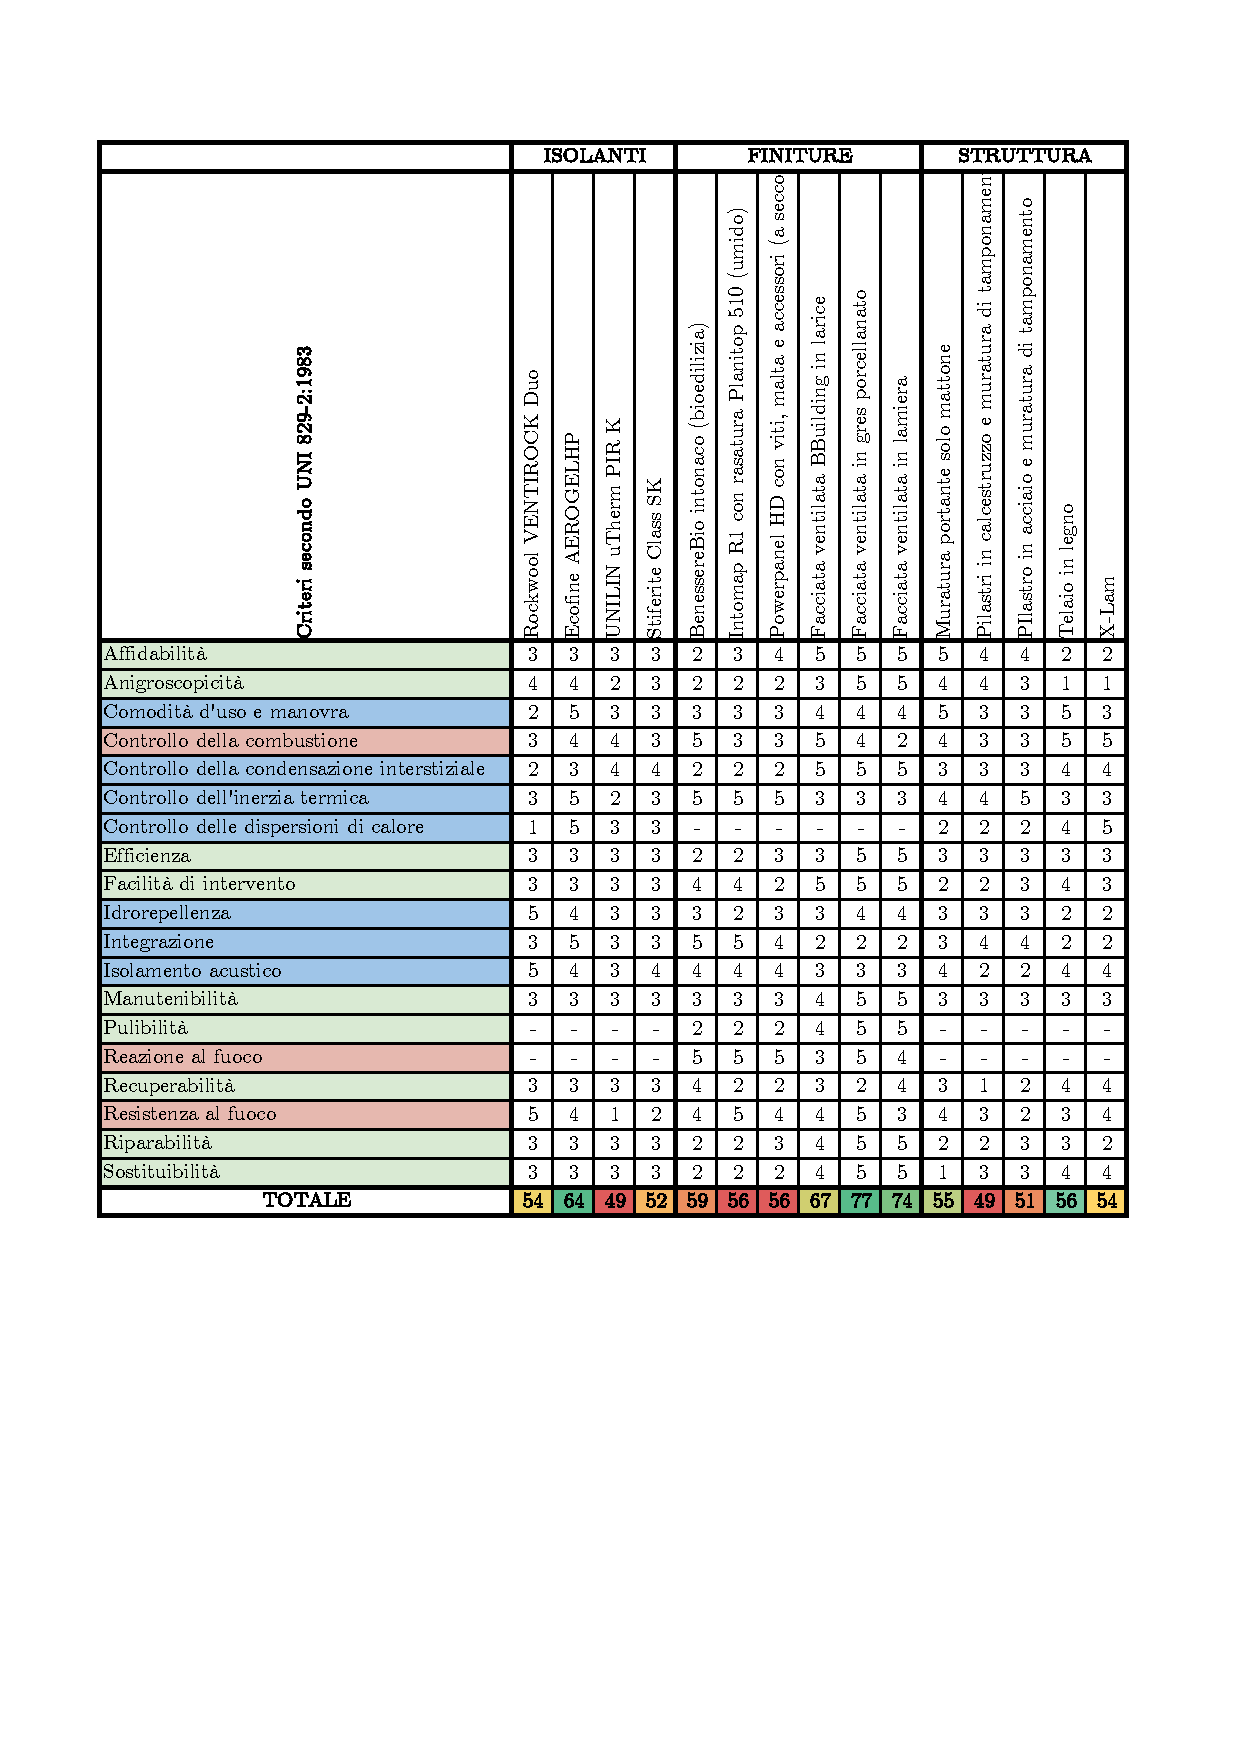
\includegraphics[width=0.9\textwidth]{img/AnalisiValore.pdf}
    \caption[Analisi del valore delle pareti esterne]{%
\scriptsize
Analisi del valore delle pareti esterni in cui è stato dato un punteggio da 1 a 5 per ogni campo considerato.
\textbf{Affidabilità:} Capacità di mantenere sensibilmente invariata nel tempo la propria qualità in condizioni d'uso determinate
\textbf{Anigroscopicità:} Attitudine a non subire mutamenti di aspetto e/o morfologia, di dimensione e comportamento in seguito ad assorbimento di acqua o di vapor d'acqua
\textbf{Comodità d'uso e manovra:} Attitudine a presentare opportune caratteristiche di funzionalità, di facilità d'uso, di manovrabilità
\textbf{Controllo della combustione:} Realizzazione e mantenimento di condizioni tali da produrre processi di combustione a massimo rendimento di trasformazione e minima produzione di scorie e sostanze inquinanti
\textbf{Controllo della condensazione interstiziale:} Attitudine ad evitare la formazione di acqua di condensa all'interno degli elementi
\textbf{Controllo dell'inerzia termica:} Attitudine ad attenuare entro opportuni valori l'ampiezza di oscillazione della temperatura e a ritardarne di una opportuna entità l'effetto
\textbf{Controllo delle dispersioni di calore:} Contenimento entro determinati livelli delle perdite di calore per conduzione, convezione e irraggiamento
\textbf{Efficienza:} Capacità costante di rendimento nel funzionamento
\textbf{Facilità di intervento:} Possibilità di operare ispezioni, manutenzione e ripristini in modo agevole
\textbf{Idrorepellenza:} Attitudine a non essere penetrato da fluidi liquidi
\textbf{Integrazione:} Attitudine alla connessione funzionale e dimensionale
\textbf{Isolamento acustico:} Attitudine a fornire un'adeguata resistenza al passaggio di rumori
\textbf{Manutenibilità:} Possibilità di conformità a condizioni prestabilite entro un dato periodo di tempo in cui è compiuta l'azione di manutenzione
\textbf{Pulibilità:} Attitudine a consentire la rimozione di sporcizia e sostanze indesiderate
\textbf{Reazione al fuoco:} Grado di partecipazione di un materiale combustibile ad un fuoco al quale è sottoposto
\textbf{Recuperabilità:} Attitudine alla riutilizzazione di materiali o di elementi tecnici dopo demolizione o rimozione
\textbf{Resistenza al fuoco:} Attitudine a conservare, entro limiti determinati, per un intervallo di tempo determinato, le prestazioni fornite
\textbf{Riparabilità:} Attitudine a ripristinare l'integrità, la funzionalità e l'efficienza di parti o oggetti guasti 
\textbf{Sostituibilità:} Attitudine a consentire la collocazione di elementi tecnici al posto di altri}
\label{fig:AnalisiValore}
\end{figure}